\documentclass[journal,twocolumn,12pt]{ieeesyscoin}
\usepackage{cite}
\usepackage{amsmath,amssymb,amsfonts}
\usepackage{algorithmic}
\usepackage{enumitem}
\usepackage{caption}
\usepackage{xcolor}
\usepackage{graphicx}
\usepackage{textcomp}
\usepackage{multirow}
\usepackage{lipsum}
\usepackage{makecell}
\usepackage[switch]{lineno}
\def\BibTeX{{\rm B\kern-.05em{\sc i\kern-.025em b}\kern-.08em
    T\kern-.1667em\lower.7ex\hbox{E}\kern-.125emX}}
\begin{document}

\history{}

\title{\centering An Analytical and Empirical Survey of Impermanent Loss}
\author{\centering \uppercase{Ian C. Moore, PhD}\authorrefmark{1},and
\uppercase{Jagdeep Sidhu, MSc}\authorrefmark{2}}

\address[1]{\centering  Syscoin Researcher, Syscoin Platform (e-mail: imoore@syscoin.org)}
\address[2]{\centering Syscoin Lead Developer, (e-mail: sidhujag@syscoin.org)}
\tfootnote{}

\markboth
{Moore \headeretal: An Analytical and Empirical Survey of Impermanent Loss}
{Moore \headeretal: An Analytical and Empirical Survey of Impermanent Loss}

\corresp{}

\begin{abstract}
\lipsum[1]
\end{abstract}

\begin{keywords}
DAOSYS, Smart DAO, Decentralized Finance, Hyper-diamond proxy, EIP-2535
\end{keywords}

\titlepgskip=-15pt

\maketitle

\section{Introduction}
\label{sec:introduction}

\lipsum[1]


\section{Analytical Survey}

\subsection{Expected Impermanent Loss}
\label{sec:exp_impermanent_loss}



Impermanent (divergence) Loss  (IL), is derived as:
\begin{equation}\label{eqn:imp_loss}
IL = \frac{V_{0} - V_{H}}{V_{H}} 
\end{equation}
where $V_{0}$ is the initial value of the portfolio holding,
\begin{equation}\label{eqn:initial_lp_value}
V_{0} = 2L\sqrt{P_{0}\alpha}
\end{equation}
where $L$ is the liquidity, $P_{0}$ is the initial price, and $\alpha$ is the price ratio (i.e., $\frac{p_{0}}{p_{f}}$) 
and $V_{H}$ is the held portfolio value, and is derived by the following:
\begin{equation}\label{eqn:held_lp_value}
V_{H} = 2L\sqrt{P_{0} (1+\alpha)}
\end{equation}
Eq. (\ref{eqn:imp_loss}) can be derived as shown in XX to provide:
\begin{equation}\label{eqn:imp_loss_derv}
IL = \frac{2\sqrt{\alpha}}{1+\sqrt{\alpha}} - 1
\end{equation}

However, (\ref{eqn:imp_loss}) provides limited insight, as it is represented only in terms of the price ratio, $\alpha$, which provides no insight when considering the stochastic nature of the price behaviour itself. To provide this we assume that price assets move in a Geometric Brownian Motion (GBM) as first provided in \cite{Gui21}; see Appendix \ref{sec:gbm}. When representing IL stochastically, its expectation can be derived as:

\begin{equation}\label{eqn:exp_imp_loss}
  E\{IL\} = \frac{e^{-\frac{\sigma^2 t}{8}}}{\cosh (\frac{\mu t}{2})} - 1.
\end{equation}
Eq. (\ref{eqn:exp_imp_loss}) was first found in \cite{Gui21}, but with no derivation or explanation on how it was derived, however \cite{Dan22} provided a good elaboration on it's derivation, but with missing steps. See Appendix \ref{sec:exp_imp_loss_derv} for a full analytical derivation of (\ref{eqn:exp_imp_loss}) where the remaining steps are provided.



\begin{figure}[h!]
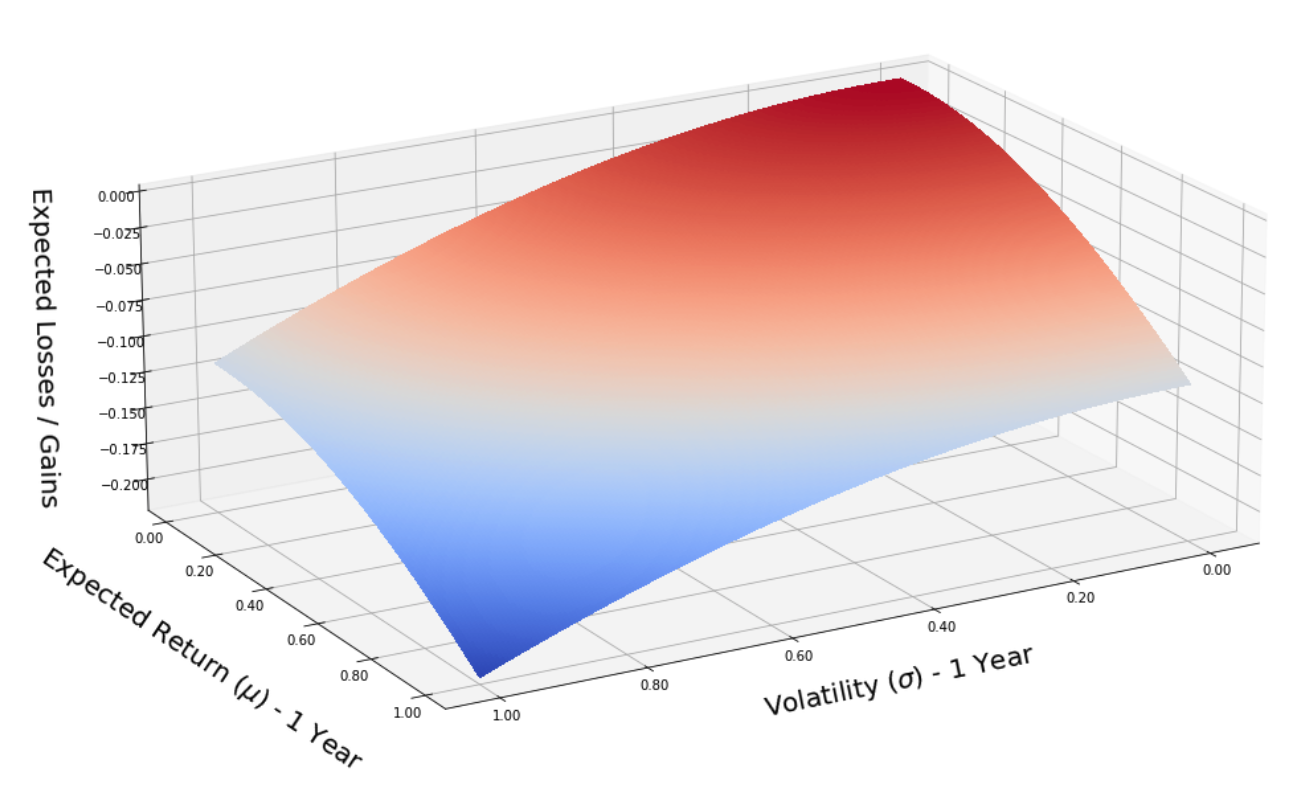
\includegraphics[width=3in]{img/imp_loss.png}
\caption{Expected impermanent loss for first year (ie, t = 1)} 
\label{fig:daosys_protocol}
\end{figure}

\subsection{Expected Portfolio Values}
\label{sec:exp_portfolio_value}

\lipsum[1]

\begin{equation}\label{eqn:held_portfolio}
  E\{V_{H}\} = 2 L \sqrt{P_{0}} (1 + e^{\mu t})
\end{equation}

\begin{equation}\label{eqn:portfolio_outside}
  E\{V\} = 2 L \sqrt{P_{0}}  e^{(\frac{\mu t}{2} - \frac{\sigma^2 t}{8})}
\end{equation}

\subsection{Expected Returns with Compounding Fees}
\label{sec:exp_lp_returns}

\lipsum[1]

\begin{equation}\label{eqn:portfolio_outside}
  E\{V\} = 2 L \sqrt{P_{0}}  e^{(\frac{\mu t}{2} - \frac{\sigma^2 t}{8})}e^{z_{t}}
\end{equation}

\begin{equation}\label{eqn:exp_returns}
  E\{R\} = \frac{e^{-\frac{\sigma^2 t}{8} + z_{t}}}{\cosh (\frac{\mu t}{2})}
\end{equation}
Referring to (\ref{eqn:portfolio_outside}) and (\ref{eqn:exp_returns}), the term $e^{z_{t}}$ represents portfolio growth due to the accumulation of trading fees, where $z_{t}$ can be defined a myriad of ways. If we take the aggregation of individual deposits $a_{i}$ over each $t$ in the form of a geometric mean, this can be expressed by the following:

\begin{equation}\label{eqn:geo_mean}
  (\prod_{i=1}^{n}a_{i})^{\frac{1}{n}} = e^{\frac{1}{n}\sum_{i}^{n}\ln a_{i}}
\end{equation}
For sake of brevity, we assume $\alpha = \frac{1}{n}\sum_{i}^{n}\ln a_{i}$, hence the growth term becomes:
\begin{equation}\label{eqn:geo_mean}
  F_{t} = e^{\alpha t}
\end{equation}
where $\alpha$ represents constant rate of growth, hence assuming GBM, the overall expected returns become:
\begin{equation}\label{eqn:exp_returns}
  E\{R\} = \frac{e^{-\frac{\sigma^2 t}{8} + \alpha t}}{\cosh (\frac{\mu t}{2})}
\end{equation}

\begin{figure}[h!]
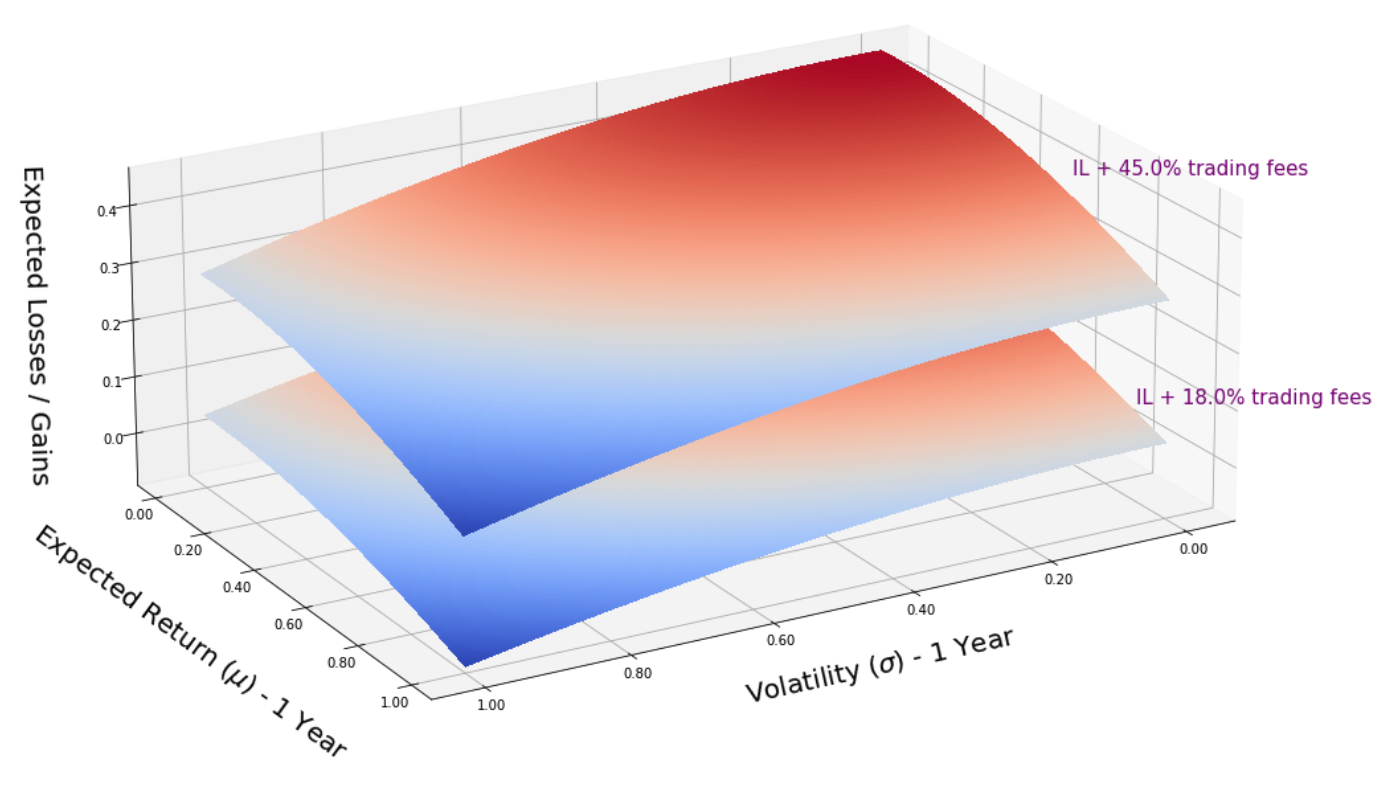
\includegraphics[width=3in]{img/imp_loss_compounding_fees.png}
\caption{Expected impermanent loss with compounding trading fees for first year (ie, t = 1)} 
\label{fig:daosys_protocol}
\end{figure}

\section{DeFi Python Simulator}
\label{sec:python_simulator}

To realize proper tokenomics design, it is highly inefficient to invest resources into development without first conducting a proper simulations of the design to test specifications for various outcomes. This is what every DeFi project in the crypto space is not doing. This is why we are introducing an open source python package to simulate various sandboxed DeFi components of DAOSYS so that project engineers, managers and designers can pre-plan outcomes prior to investing valuable resources into development.

With this tool, DAOSYS designers can utilize the plug and play components of our simulator to build tokenomics mockups for business planning purposes so that teams can come together and get collective consensus alongside potential users and investors. Not only is this tool applicable to DAOSYS, it can be used as a general purpose tool to simulate DEX activity for anyone wishing to setup their own liquidity pool (LP) and wish to stress test their ideas prior to development. This can be used as a powerful design tool to explore the limitations of an DeFi project idea prior to committing valuable resources on development costs (ie, Devs and Project Managers). Table \ref{table:simulator_components} highlights the main components of the simulator, so that potential users of the system can get a higher level understanding of the DeFi simulator package.

\begin{table}[h]
\centering
\begin{tabular}{ |l|l| } 
\hline
 \textbf{Simulator Component} & \textbf{Description} \\
\hline
Agents          & Entities that engage with the system, and are  \\
                & subcategorized into tokens and users \\
Events          & Agnostic events that take place within the \\ 
				& system (eg, mint, deposit, withdraw, swap, \\
				& and rebase) \\
ModelQueue      & Queue of univariate events that are modelled \\
				& aprior that can be fed into the system as \\
				& events\\
Actions         & Event actions that are fed into the system \\
				& performed by agents; they can either be single \\
				& stand-alone independent event actions or \\
				& chained together with dependency \\
ActionChains    & Actions that have dependencies on other \\
				& actions as inputs \\				
ActionBatch     & Batches of actions placed together into a \\
				& repeatable sequence; there is only one \\
				& assigned time delta per the pass of each batch, \\
				& and there is no limit as to the number of \\
				& batches that can be created \\
Liquidity Pools & Pool of two token agents managed by constant \\ 
				& product trading \\
Orchestrator    & Manages agents and actions working within the \\ 
				& system \\
Event Queue     & Queue of storable actions \\
Event Executor  & Final step which executes queue of action \\
				& events \\
\hline
\end{tabular}
\caption{Descriptions of DeFi python simulator components; refer to Fig. \ref{fig:simulator} to see how components interact with one another.}
\label{table:simulator_components}
\end{table}

We have a working beta version of the simulator which is available through Syscoin’s Github repository. This simulator is being built alongside DAOSYS, and we are using this to understand the ROI and design considerations for DAOSYS’s first usecase (ie, Masternode Yield Farming). Since the simulator is still in the beta stage, the setup is currently not realized to its full intention. However, a downloadable demo of this tool is available from Syscoin's Github repository for the community to begin using. For a mini python tutorial on how to use this tool, please refer to \cite{Moo22B} and refer to \cite{DAOSim22} for a series of example Jupyter notebooks.

The purpose of this tool is primarily for the design aspect of DAOSYS, and is still in its early stages of development. The next stages involve feeding the output of various mathematical models into the simulator framework and to use this tool to simulate other DeFi usecases. This is so that we can test a roster of edge cases to build more robust systems. The final goal is to bring this system to a level of maturity so that it can be utilized in parallel with the contracts in real time. Hence, exposing DeFi to a scientific way of design, testing, and implementation.

\begin{figure}[h!]
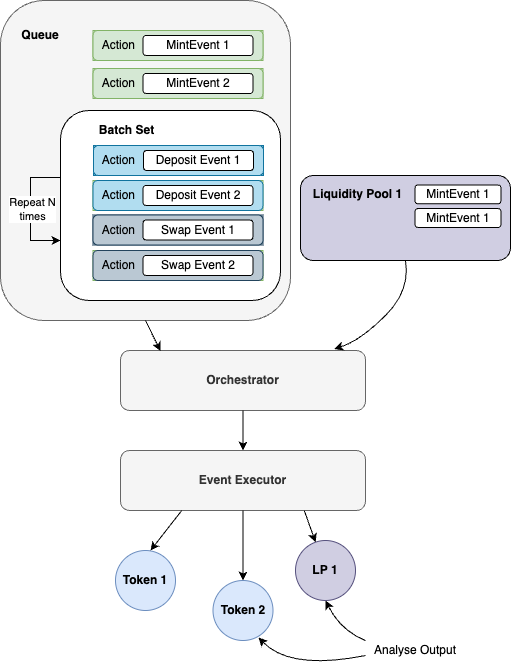
\includegraphics[width=3in]{img/simulator.png}
\caption{System components to DeFi Python simulator for DAOSYS} 
\label{fig:simulator}
\end{figure} 

\section{Numerical Simulations}
\label{sec:numerical_simulations}

\lipsum[1]


\begin{figure}[h!]
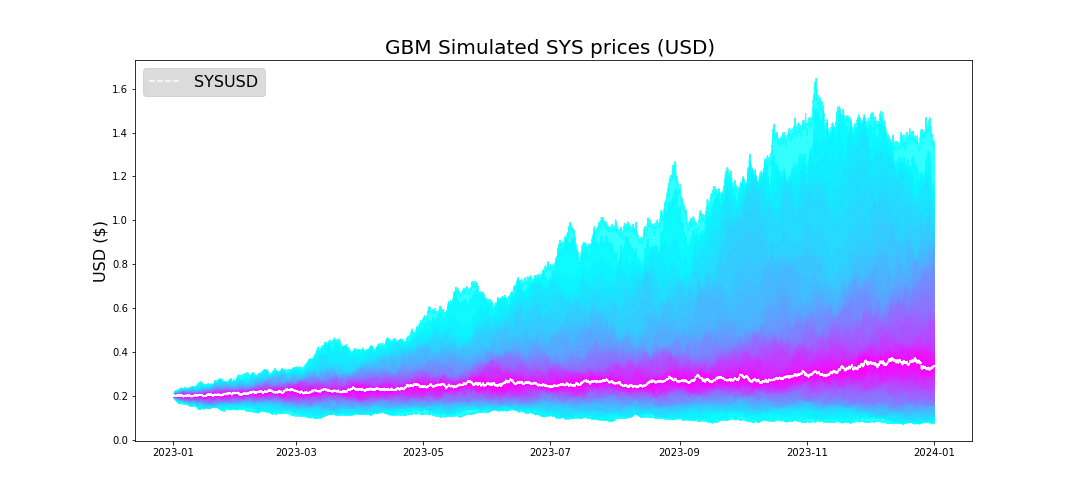
\includegraphics[width=3in]{img/price_simulations.png}
\caption{xxx} 
\label{fig:daosys_protocol}
\end{figure}


\begin{figure}[h!]
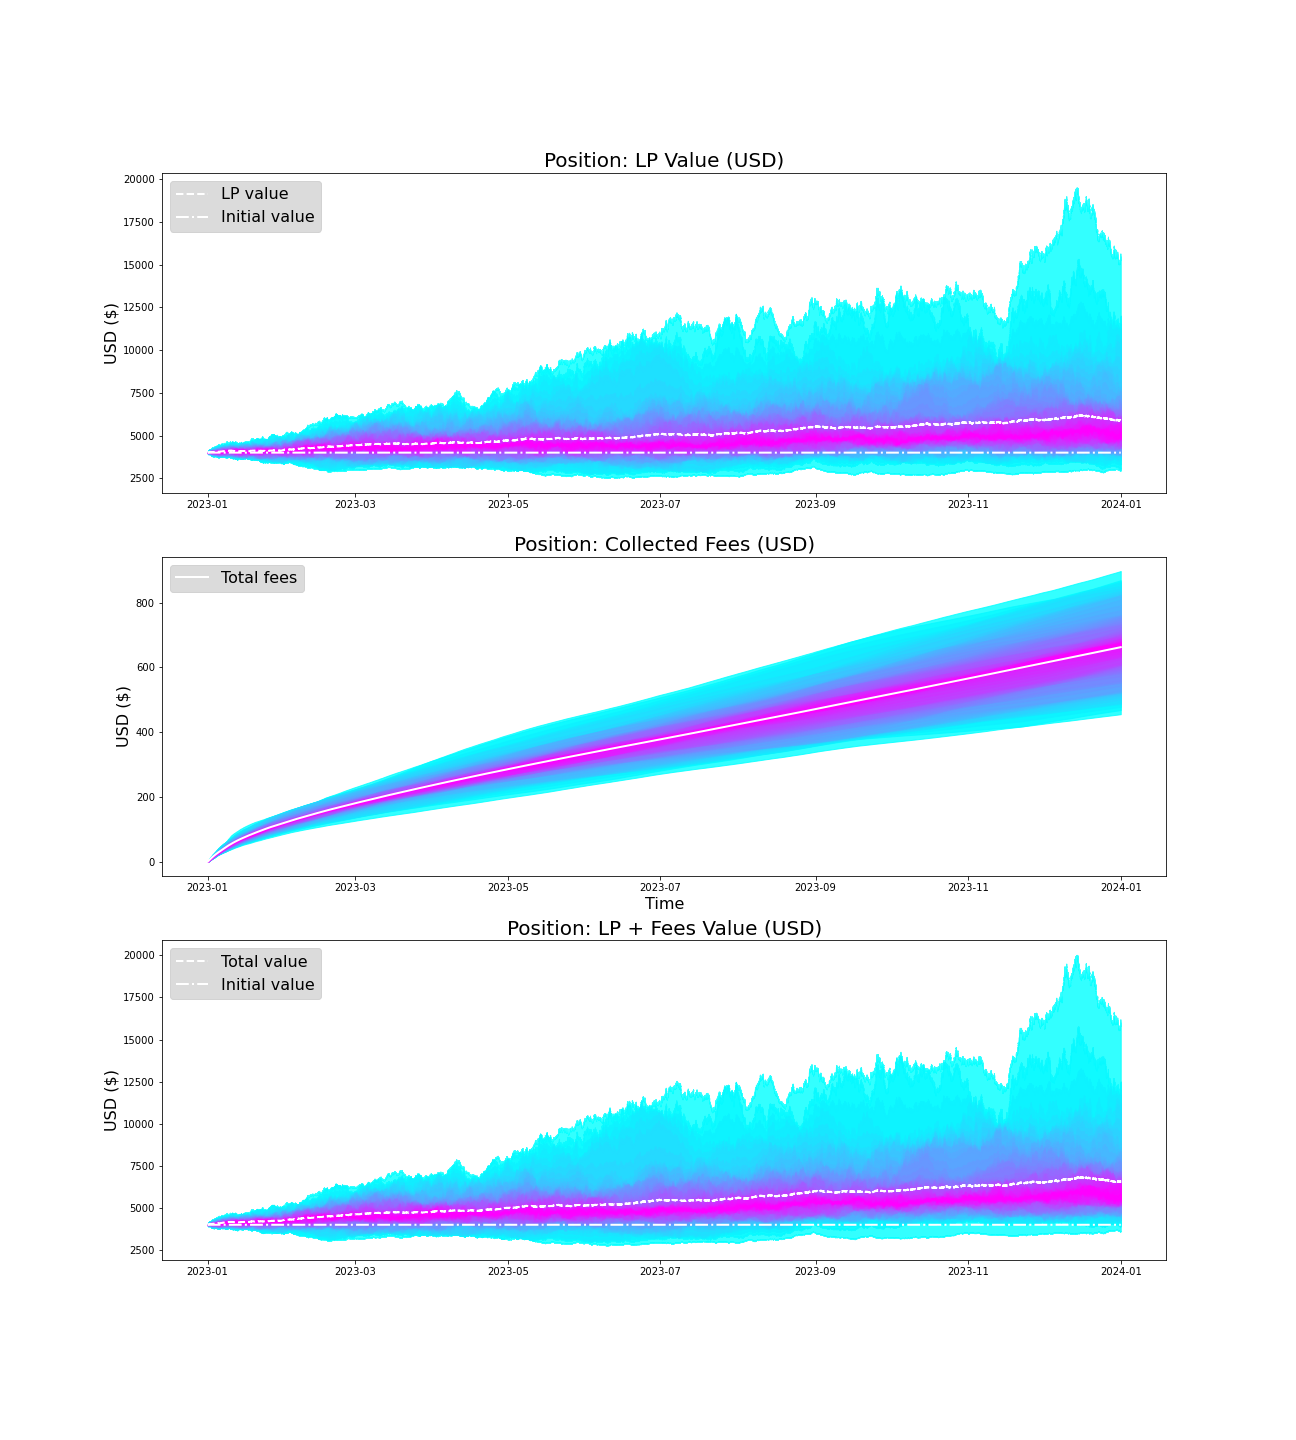
\includegraphics[width=3in]{img/lp_position_values.png}
\caption{xxx} 
\label{fig:daosys_protocol}
\end{figure}


\begin{figure}[h!]
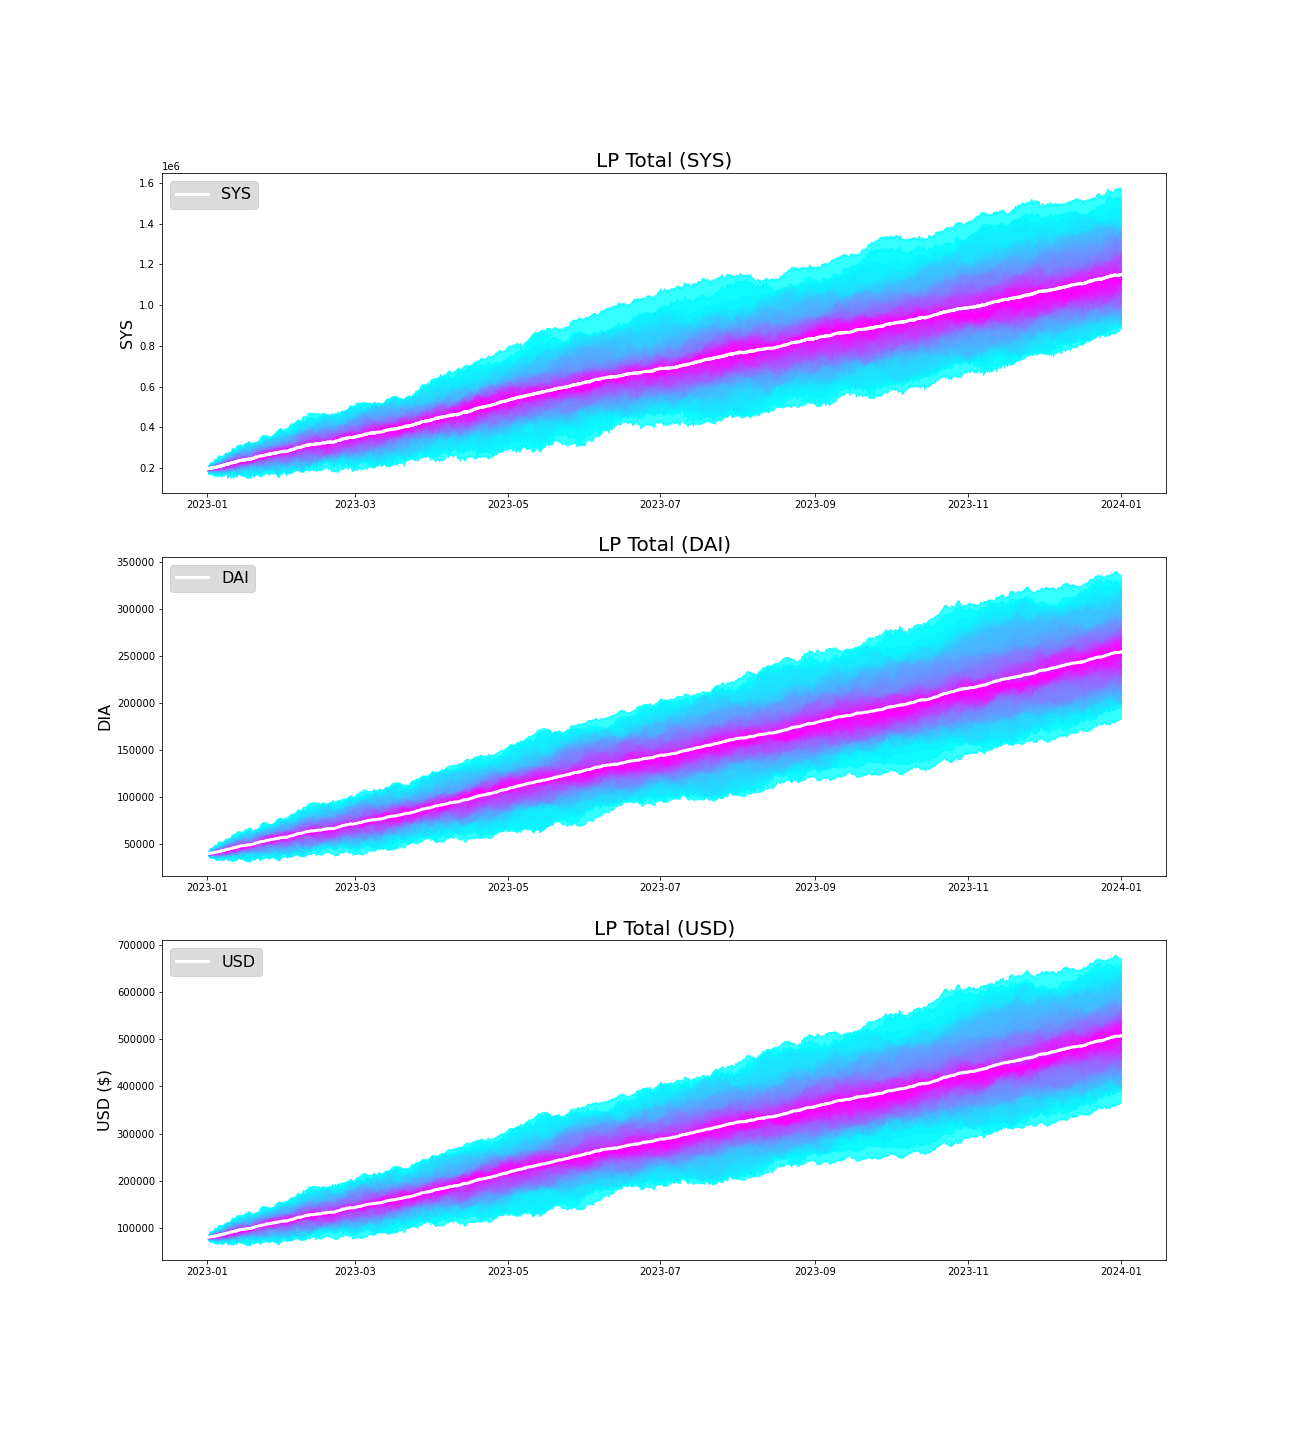
\includegraphics[width=3in]{img/lp_simulation.png}
\caption{xxx} 
\label{fig:daosys_protocol}
\end{figure}

\section{Summary}
\label{section:summary}

\lipsum[1]

\begin{table}[h!]
\centering
\begin{tabular}{|c|c ||c|c||c|c||c|c| } 
\hline
\multicolumn{2}{|c}{ }  & \multicolumn{2}{c }{ Fees (\%) } & \multicolumn{2}{c}{ Imp Loss (\%)}  & \multicolumn{2}{c|}{ Gain / Loss (\%)}\\
$\mu$ & $\sigma$ & Theo.  & Sim. & Theo.& Sim.& Theo. & Sim. \\
\hline
 \multirow{3}{*}{0.4} & \multirow{3}{*}{0.5} & 4.75  & 4.86 & -4.98 & -4.79 & -0.36  & -0.78 \\
                          &  &  5.15 & 5.28 & -4.98  & -4.13  & 0.04 & 0.20 \\
                          &  &  5.33 & 5.47 & -4.98  & -3.93 & 0.22  & 0.69   \\
\hline
\multirow{ 3}{*}{0.1} & \multirow{3}{*}{0.1} & 3.28  & 3.33 & -0.25 & -0.29 & 3.07  & 2.84 \\
                          &  &  3.09 & 3.13 & -0.25 & -0.22 & 2.88 & 2.78 \\
                          &  &  3.17 & 3.22 & -0.25 & -0.21 & 2.96 & 2.90  \\
\hline
\multirow{ 3}{*}{0.8} & \multirow{3}{*}{0.4} & 5.14  & 5.28 & -9.33 & -9.58 & -4.55 & -6.29\\
                           &  & 4.74  & 4.85 &  -9.33  & -7.33 &   -4.93  &  -4.38  \\
                           &  & 4.78  & 4.90 & -9.33  & -6.88 &  -4.89 & -3.82   \\
\hline
\end{tabular}
\caption{Low liquidity (num intervals = 5,000)}
\label{table:sim_vs_theory1}
\end{table}

\begin{table}[h!]
\centering
\begin{tabular}{|c|c ||c|c||c|c||c|c| } 
\hline
\multicolumn{2}{|c}{ }  & \multicolumn{2}{c }{ Fees (\%) } & \multicolumn{2}{c}{ Imp Loss (\%)}  & \multicolumn{2}{c|}{ Gain / Loss (\%)}\\
$\mu$ & $\sigma$ & Theo.  & Sim. & Theo.& Sim.& Theo. & Sim. \\
\hline
\multirow{3}{*}{0.4} & \multirow{3}{*}{0.5} & 8.82  & 9.22 & -4.98 & -5.79 & 3.78  & 1.34 \\
                          &  &  8.72 & 9.12 &  -4.98 & -6.07  & 3.68 & 1.25 \\
                          &  & 8.49  &  8.86 & -4.98 &  -3.80 & 3.43  &  3.82  \\
\hline
\multirow{ 3}{*}{0.1} & \multirow{3}{*}{0.1} & 5.45  & 5.60 &  -0.25 & -0.23 & 5.33 & 5.08 \\
                          &  & 5.41 & 5.56 &  -0.25  & -0.19 & 5.29  & 5.12  \\
                          &  & 5.22  & 5.36 & -0.25  & -0.27 &  5.09 & 4.80   \\
\hline
\multirow{ 3}{*}{0.8} & \multirow{3}{*}{0.4} & 8.52 &  8.89 &  -9.33 & -8.75 & -1.27 & -3.22 \\
                         &  & 8.40  & 8.76 & -9.33  & -7.81 &  -1.39  &  -2.06  \\
                         &  & 8.67  & 9.06 & -9.33  & -7.84 & -1.12  &  -1.99   \\
\hline
\end{tabular}
\caption{High liquidity (num intervals = 25,000)}
\label{table:sim_vs_theory2}
\end{table}


\appendices

\section{Geometric Brownian Motion}
\label{sec:gbm}

\begin{equation}\label{eqn:gbm}
  S_{t} = S_{0} e^{(\mu - \frac{\sigma^2}{2})t  + \sigma W_{t} }
\end{equation}

\lipsum[1]

\section{MGF of Brownian Motion}
\label{sec:exp_brownian_motion}

The moment generating function (MGF), $M(a)$, for a random variable X is $E\{e^{aX}\}$. Thus, the MGF of a normal random variable is given by:
\begin{eqnarray*}\label{eqn:mgf_normal}
M(a) &=& E\{e^{aX}\}\\ 
           &=& \int_{-\infty}^{\infty}e^{ax}f(x)dx \\
           &=& e^{a\mu + \frac{1}{2}a^2\sigma^2}
\end{eqnarray*}
where $X \sim N(\mu, \sigma^2)$. Since a standard Brownian motion process, $W_{t}$, is also normally distributed where $W_{t} \sim N(0,t)$, we have:

\begin{equation}\label{eqn:mgf_bm}
  E\{e^{aW_{t}}\} = e^{\frac{1}{2}a^2t}
\end{equation}

\section{Expected Impermanent Loss Derivation}
\label{sec:exp_imp_loss_derv}

Under the assumption of GBM, equations (\ref{eqn:initial_lp_value}) and (\ref{eqn:held_lp_value}) can be represented as:

\begin{equation}\label{eqn:initial_lp_value_gbm}
V_{0} = 2L\sqrt{P_{0} e^{(\mu - \frac{\sigma^2}{2})t + \sigma W_{t} } },
\end{equation}

and  

\begin{equation}\label{eqn:held_lp_value_gbm}
V_{H} = 2L\sqrt{P_{0}} ( 1 + e^{(\mu - \frac{\sigma^2}{2})t + \sigma W_{t} } ).
\end{equation}
Using (\ref{eqn:initial_lp_value_gbm}) and the MGF of standard Brownian motion from (\ref{eqn:mgf_bm}), we first can calculate $E\{V_{0}\}$:

\begin{eqnarray*}\label{eqn:derivation_exp_v0}
E\{V_{0}\} &=& E\{2L \sqrt{P_{0}} e^{(\frac{\mu}{2} - \frac{\sigma^2}{4})t } e^{\frac{\sigma W_{t}}{2}} \} \\ 
           &=& 2L \sqrt{P_{0}} e^{(\frac{\mu}{2} - \frac{\sigma^2}{4})t } E\{e^{ \frac{\sigma W_{t}}{2} }\} \\
           &=& 2L \sqrt{P_{0}} e^{(\frac{\mu}{2} - \frac{\sigma^2}{4})t } e^{\frac{\sigma^2 t}{8}} \\
           &=&  2L \sqrt{P_{0}}e^{( \frac{\mu}{2} - \frac{\sigma^2}{8})}
\end{eqnarray*}
Likewise, using (\ref{eqn:held_lp_value_gbm}) and the same MGF of standard Brownian motion from (\ref{eqn:mgf_bm}), we calculate $E\{V_{H}\}$: 
\begin{eqnarray*}\label{eqn:derivation_exp_vH}
E\{V_{H}\} &=& E\{L \sqrt{P_{0}}(1 + e^{(\mu - \frac{\sigma^2}{2})t + \sigma W_{t} })\} \\
		   &=& L \sqrt{P_{0}}(1 + E\{ e^{(\mu - \frac{\sigma^2}{2})t + \sigma W_{t} }  \}) \\
		   &=& L \sqrt{P_{0}}(1 + e^{(\mu - \frac{\sigma^2}{2})t} E\{e^{\sigma W_{t}}\} ) \\
		   &=& L \sqrt{P_{0}}(1 + e^{(\mu - \frac{\sigma^2}{2})t} e^{\frac{\sigma^2}{2}t} \\
		   &=& L \sqrt{P_{0}}(1 + e^{\mu t} )
\end{eqnarray*}
Therefore using the the identity $\cosh(x) = \frac{1 + e^{2x}}{2 e^x}$, and our definition of IL outlined in (\ref{eqn:imp_loss})  we have:
\begin{eqnarray*}\label{eqn:derivation_exp_IL}
E\{IL\} &=& \frac{E\{V_{0}\} - E\{V_{H}\}}{E\{V_{H}\}} \\
		&=& \frac{2L \sqrt{P_{0}}e^{( \frac{\mu}{2} - \frac{\sigma^2}{8})} }{L \sqrt{P_{0}}(1 + e^{\mu t} )}\\
		&=& \frac{2e^{( \frac{\mu}{2} - \frac{\sigma^2}{8})}}{1 + e^{\mu t}} - 1\\
		&=& \frac{e^{-\frac{\sigma^2 t}{8}}}{ cosh(\frac{\mu t}{2})} - 1
\end{eqnarray*}


\section{Simulated LP Asset Balances}
\label{sec:sim_lp_balances}
Here we address the problem of updating asset balances (ie, $x_{t}$,$y_{t}$) upon each price change $\Delta p_{t}$, where $p_{t}$ is a simulated GBM process representing the prices of our asset class in USD over time $t$. Price change, $\Delta p_{t}$, in a liquidity pool are determined as:

\begin{eqnarray*}\label{eqn:deltap1}
\Delta p_{t} &=& \frac{y_{t}}{x_{t}} - \frac{y_{t-1}}{x_{t-1}} \\
			 &=& \frac{\Delta y_{t} + y_{t-1}}{\Delta x_{t} + x_{t-1}} - \frac{y_{t-1}}{x_{t-1}}
\end{eqnarray*}
and asset trade price is determined as: 
\begin{equation}\label{eqn:deltap2}
  p_{t} = \frac{\Delta y_{t}}{\Delta x_{t}}
\end{equation}
Thus, given the above equations, we derive the following system of non-linear equations:
\begin{eqnarray}\label{eqn:non_linear_system}
\frac{x_{t-1} \Delta y_{t-1} - \Delta x_{t} y_{t-1}}{x_{t-1}^2 + x_{t-1} \Delta x_{t}} - \Delta p_{t} &=& 0 \\
\frac{\Delta y_{t}}{\Delta x_{t}} - p_{t} &=& 0.
\end{eqnarray}
Since we have the previous balances $y_{t-1}$, $x_{t-1}$, price change $\Delta p_{t}$ and the current price $p_{t}$ from our simulated GBM, we can solve for the swap balances $\Delta x_{t}$ and $\Delta y_{t}$ under the constraints $\Delta y_{t} > 0$ and $\Delta x_{t} > 0$ for every $t$. To achieve this, we used the \verb|optimize.fsolve| function from \verb|scipy| package in python. 


\begin{thebibliography}{00}

\bibitem{Pin19a} Pintail, \textit{Uniswap: A Good Deal for Liquidity Providers?}, Jan. 2019. Accessed on: Dec 2022.  [Online]. Available:  https://pintail.medium.com/uniswap-a-good-deal-for-liquidity-providers-104c0b6816f2

\bibitem{Pin19b} Pintail, \textit{Understanding Uniswap Returns}, Feb. 2019. Accessed on: Dec 2022.  [Online]. Available:  hhttps://pintail.medium.com/understanding-uniswap-returns-cc593f3499ef

\bibitem{Pet21} P. Erins, \textit{How to calculate Impermanent Loss: full derivation}, Jun. 2021. Accessed on: Dec 2022.  [Online]. Available:  https://medium.com/auditless/how-to-calculate-impermanent-loss-full-derivation-803e8b2497b7

\bibitem{Aig21} A. Aigner and G. Dhaliwal, \textit{UNISWAP: Impermanent Loss and Risk Profile of a Liquidity Provider}, Jun. 2021. Accessed on: Dec 2022.  [Online]. Available:  https://arxiv.org/pdf/2106.14404.pdf

\bibitem{Gui21} G. Lambert, \textit{Calculating the Expected Value of the Impermanent Loss in Uniswap}, Oct. 2021. Accessed on: Dec 2022.  [Online]. Available:  https://lambert-guillaume.medium.com/an-analysis-of-the-expected-value-of-the-impermanent-loss-in-uniswap-bfbfebbefed2

\bibitem{Dan22} Danr, \textit{Expected Impermanent Loss in Uniswap V2 \& V3}, Mar. 2022. Accessed on: Dec 2022.  [Online]. Available:  https://medium.com/gammaswap-labs/expected-impermanent-loss-in-uniswap-v2-v3-7fb81033bd81

\bibitem{Dec21} Danr, \textit{Total Returns and Impermanent Loss in Uniswap V2}, Dec. 2021. Accessed on: Dec 2022.  [Online]. Available:  https://medium.com/gammaswap-labs/total-returns-and-impermanent-loss-in-uniswap-v2-9f3d5b6ebc89


\bibitem{Uni19} Uniswap Blog, \textit{A short history of Uniswap}, Sept. 2019. Accessed on: Sept 2022.  [Online]. Available:  https://uniswap.org/blog/uniswap-history

\bibitem{Moo22A} I.C. Moore,  \textit{Masternode Yield Farming as a DAOSYS Usecase: Part 1}, Medium Article, Aug. 2022. Accessed on: Sept 2022.  [Online]. https://icmoore.medium.com/masternode-yield-farming-as-a-daosys-usecase-part-1-8485ab7ba721

\bibitem{Moo22B} I.C. Moore,  \textit{Masternode Yield Farming as a DAOSYS Usecase: Part 2}, Medium Article, Aug. 2022. Accessed on: Sept 2022.  [Online]. https://icmoore.medium.com/masternode-yield-farming-as-a-daosys-usecase-part-2-8906d0a11c27

\bibitem{DAOSim22} I.C. Moore, \textit{Simulation: Masternode Yield Farming}, Syscoin Github repos, Accessed on: Apr 2021.  [Online]. Available: https://github.com/syscoin/daosys/tree/main/notebooks/simulation

\bibitem{ROL22} Syscoin News, \textit{Introducing Rollux, Syscoin's Rollup Suite Ready to Take Market by Storm}, Syscoin, Jun. 2022. Accessed on: Sept 2022.  [Online]. Available: https://syscoin.org/news/introducing-rollux-syscoins-rollup-suite-ready-to-take-market-by-storm

\bibitem{Sig21a} J. Sidhu, \textit{A Design For An Efficient Coordinated Financial Computing Platform}, Feb 2021, Accessed on: Sep 2021.  [Online]. Available:  https://jsidhu.medium.com/a-design-for-an-efficient-coordinated-financial-computing-platform-ab27e8a825a0

\bibitem{Sig21b} J. Sidhu and I.C. Moore, \textit{Syscoin 4: A Peer-to-Peer Electronic Cash System Built For Decentralized
Web 3.0 Business Applications}, Syscoin Platform, Dec. 2021. Accessed on: Sept 2022. [Online]. Available: https://syscoin.org/$syscoin4\_whitepaper.pdf$



\end{thebibliography}


\EOD

\end{document}
